\documentclass{clbeamer2024}

\usepackage{minted}

\usepackage{minted}
\setminted{
	breaklines=true,
	frame=single,
	bgcolor=lightgray,
	fontsize=\small,
	escapeinside=||
}

\usepackage{xcolor}
\definecolor{bg}{rgb}{0.95, 0.95, 0.92} % Couleur gris clair

\title{
	%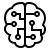
\includegraphics[width=0.5cm]{logos/IA1.png} \hfill
        Introduction à la Théorie de la Compilation
	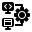
\includegraphics[width=0.7cm]{logos/compilation.png} \hfill
}
\subtitle{Comprendre les bases de la création de compilateurs}
\author{Slimani Mohamed Amine}
\institute{EHTP}
\date{\today}

\begin{document}
	\setcounter{framenumber}{-1}
	\frame{\titlepage}
	
	
	
	% Sommaire
	\begin{frame}{Sommaire}
		\tableofcontents
	\end{frame}
	
	
	\section{Qu'est-ce que la compilation ?}
	\begin{frame}{Qu'est-ce que la compilation ?}
		\begin{itemize}
			\item \textbf{Définition} : La compilation est le processus de traduction d'un programme écrit dans un langage de haut niveau en un langage de bas niveau (ex : assembleur, code machine).
			\item \textbf{Objectif} : Produire un programme exécutable à partir du code source.
			\item \textbf{Phases de la compilation} : Analyse lexicale, analyse syntaxique, analyse sémantique, génération de code, optimisation.
		\end{itemize}
	\end{frame}
	
	\section{Pourquoi la théorie de la compilation est-elle importante ?}
	\begin{frame}{Pourquoi la théorie de la compilation est-elle importante ?}
		\begin{itemize}
			\item \textbf{Compréhension des langages} : Comprendre comment les langages de programmation fonctionnent.
			\item \textbf{Optimisation} : Améliorer les performances des programmes.
			\item \textbf{Création de compilateurs} : Développer des compilateurs pour de nouveaux langages.
		\end{itemize}
	\end{frame}
	
	\section{Phases de la compilation}
	\begin{frame}{Phases de la compilation}
		\begin{itemize}
			\item \textbf{Analyse lexicale} : Convertir le code source en une séquence de tokens.
			\item \textbf{Analyse syntaxique} : Vérifier la structure syntaxique du programme.
			\item \textbf{Analyse sémantique} : Vérifier la signification du programme.
			\item \textbf{Génération de code} : Produire du code de bas niveau.
			\item \textbf{Optimisation} : Améliorer l'efficacité du code généré.
		\end{itemize}
	\end{frame}
	
	\section{Outils et technologies}
	\begin{frame}{Outils et technologies}
		\begin{itemize}
			\item \textbf{Lex} : Générateur d'analyseurs lexicaux.
			\item \textbf{Yacc} : Générateur d'analyseurs syntaxiques.
			\item \textbf{LLVM} : Infrastructure pour la génération de code et l'optimisation.
		\end{itemize}
	\end{frame}
	
	
	
	\section{Exemple d'analyse lexicale}
	\begin{frame}[fragile]{Exemple d'analyse lexicale}
		\begin{exampleblock}{Code source et tokens}
			\begin{minted}[fontsize=\scriptsize]{c}
int main() {
	return 0;
}
	\end{minted}
			\begin{minted}[fontsize=\scriptsize]{text}
KEYWORD(int) IDENTIFIER(main) SYMBOL(() SYMBOL()) SYMBOL({) KEYWORD(return) NUMBER(0) SYMBOL(;) SYMBOL(})
			\end{minted}
		\end{exampleblock}
	\end{frame}
	
	
	\section{Exemple d'analyse syntaxique}
	\begin{frame}[fragile]{Exemple d'analyse syntaxique}
		\begin{exampleblock}{Arbre syntaxique}
			\begin{minted}[fontsize=\scriptsize]{text}
FunctionDeclaration
|---Type: int
|---Name: main
|--- Parameters: ()
|--- Body:
     |---ReturnStatement
         |--- Expression: 0
			\end{minted}
		\end{exampleblock}
	\end{frame}
	
	\section{Bonnes pratiques}
	\begin{frame}{Bonnes pratiques}
		\begin{itemize}
			\item \textbf{Modularité} : Diviser le compilateur en phases distinctes.
			\item \textbf{Gestion des erreurs} : Fournir des messages d'erreur clairs et informatifs.
			\item \textbf{Optimisation} : Utiliser des techniques d'optimisation pour améliorer les performances.
		\end{itemize}
	\end{frame}
	
	\section{Défis de la compilation}
	\begin{frame}{Défis de la compilation}
		\begin{itemize}
			\item \textbf{Complexité} : Gérer la complexité des langages modernes.
			\item \textbf{Performance} : Produire du code optimisé.
			\item \textbf{Portabilité} : Générer du code pour différentes architectures.
		\end{itemize}
	\end{frame}
	
	\section{Pourquoi c'est important ?}
	\begin{frame}{Pourquoi c'est important ?}
		\begin{itemize}
			\item La théorie de la compilation est essentielle pour comprendre comment les langages de programmation sont transformés en code exécutable.
			\item Elle permet d'optimiser les performances des programmes et de créer de nouveaux compilateurs.
			\item Comprendre la théorie de la compilation est crucial pour les développeurs de compilateurs et les concepteurs de langages.
		\end{itemize}
	\end{frame}
	
	\begin{frame}{Résumé}
		\textbf{La théorie de la compilation} est une discipline clé pour la création de compilateurs et l'optimisation des programmes.  
		Explorez, apprenez, et innovez avec la compilation !
	\end{frame}


	
	
\end{document}
